% Layer derivation, selection, bridges, sub-systems

\section{Architecture}
\label{sec:architecture}

% Nine layers, evidence, selected components

\begin{table*}[!t]
\caption{Platform Layers, Their Evidence Base, and the Components Selected for Each}
\label{tab:layer_mapping}
\centering
\footnotesize
\begin{tabular}{@{}>{\raggedright\arraybackslash}p{3.0cm}>{\raggedright\arraybackslash}p{5.4cm}>{\raggedright\arraybackslash}p{1.5cm}>{\raggedright\arraybackslash}p{5.6cm}@{}}
\toprule
\textbf{Layer} & \textbf{Recurring services named by the sources} & \textbf{Sources} & \textbf{Selected open source components} \\
\midrule
Orchestration and Infrastructure & model training infrastructure, infrastructure and supporting services & \cite{kreuzberger2023mlops}, \cite{najafabadi2024analysis}, \cite{googlecloud2024mlops} & k3s, Horizontal Pod Autoscaler, Vertical Pod Autoscaler recommender, KEDA, Kueue, cert-manager \\
Data Ingestion and Processing & data collection, data cleaning, data preprocessor, data ingestion & \cite{amershi2019software}, \cite{najafabadi2024analysis}, \cite{munappy2020adhoc} & Kafka with Strimzi, Karapace, Debezium, Flink, Spark, dbt, Airflow, Trino \\
Data Storage & dataset repository, data storage, data versioning & \cite{najafabadi2024analysis}, \cite{munappy2020adhoc} & MinIO, Apache Iceberg, Lakekeeper, lakeFS, ClickHouse, PostgreSQL, MySQL, OpenSearch \\
Feature Service & feature store, offline and online serving & \cite{kreuzberger2023mlops}, \cite{googlecloud2024mlops}, \cite{najafabadi2024analysis} & Feast, ClickHouse offline, Valkey online, Qdrant on a separate index outside the Feast contract \\
Model Lifecycle & model training, model evaluation, model registry, ML metadata store, inference service & \cite{kreuzberger2023mlops}, \cite{amershi2019software}, \cite{googlecloud2024mlops}, \cite{najafabadi2024analysis} & Kubeflow Pipelines, Katib, Kubeflow Trainer, MLflow, KServe, Knative, Argo Workflows \\
Data Governance & data testing, controlled access, privacy and data integrity protection & \cite{munappy2020adhoc} & DataHub, OpenLineage, Great Expectations \\
Observability & monitoring component, model monitoring, data monitoring & \cite{kreuzberger2023mlops}, \cite{amershi2019software}, \cite{najafabadi2024analysis}, \cite{munappy2020adhoc} & Prometheus, Loki, Grafana Tempo, Grafana, OpenTelemetry, Superset, Evidently, OpenCost \\
GitOps and Continuous Delivery & CI/CD component, source code repository, deployment services & \cite{kreuzberger2023mlops}, \cite{googlecloud2024mlops}, \cite{najafabadi2024analysis} & Argo CD, Gitea, Tekton, Argo Rollouts \\
Security & controlled access, privacy and data security compliance, API gateway & \cite{munappy2020adhoc}, \cite{najafabadi2024analysis} & Istio, APISIX, dex, oauth2-proxy, SpiceDB, OpenBao, Kyverno, Falco \\
\bottomrule
\end{tabular}
\end{table*}


\subsection{Deriving the Platform Layers}
\label{subsec:layers}

The layers are derived from convergence across sources that used different methods, not from majority adoption. On the model side, Kreuzberger et al. name nine MLOps components through mixed-method research combining literature review, tool review, and expert interviews \cite{kreuzberger2023mlops}. Amershi et al. arrive at a nine-stage workflow by observing engineering teams at Microsoft, and already separate the data-oriented stages from the model-oriented ones \cite{amershi2019software}. Starting from different methods, the two name largely the same components. Amou Najafabadi et al. synthesise 35 components from 43 primary studies and report how often each occurs, with model registry at 21 occurrences, ML metadata repository at 15, and feature store at 8 \cite{najafabadi2024analysis}. Google Cloud lists seven components required for MLOps level 2 \cite{googlecloud2024mlops}.

The occurrence counts carry less weight than they suggest, because no single component reaches an absolute majority of the 43 studies. What they show is that the same components recur across independent studies.

On the data side, Munappy et al. derive an evolution model from ad-hoc analytics to DataOps from an industrial case study, naming data collection, data testing, and data monitoring as recurring practices, and treating controlled access and data-integrity protection as governance \cite{munappy2020adhoc}. The data field therefore widens the MLOps set rather than duplicating it. It is the convergence across these five sources of differing method that forms the evidence base, not a claim that any one component is used by most of the industry.

Consolidating both sides gives the nine layers in Table~\ref{tab:layer_mapping}. Four cover the data domain and five cover the model domain and platform operations. Each row traces to the sources that name its services, and the backing is not even across rows. The Model Lifecycle layer is named by four sources at once, whereas the Security layer draws mainly on the security governance dimension of the DataOps side. Table~\ref{tab:layer_mapping} leaves that difference visible instead of levelling it.

Two boundaries are deliberate. Monitoring is placed in Observability rather than in Serving, so that measurement does not mix with inference. Drift detection is not a tenth layer. It is a mechanism that crosses layers, connecting the monitoring function to the model lifecycle, and it is realised as a sub-system instead.

The layer order follows the concept order of the underlying literature study one to one, so the partitioning is not a new taxonomy standing on its own.

\subsection{Selecting Components}
\label{subsec:selection}

Every role with more than one viable candidate is scored in a comparison matrix. Each matrix scores four criteria chosen for that role, so the set is not fixed across matrices. Maturity, community size, and Kubernetes integration recur most often, while the rest are role-specific, such as batch and streaming capability for processing engines or footprint for Kubernetes distributions. Each criterion scores 0, 1, or 2, giving a maximum total of 8. A score of 0 marks a criterion that is not met, 1 marks partial support that still needs an additional component or carries a significant limitation, and 2 marks full support by built-in capability. Scores are derived from official documentation and each project's maintenance status. Twenty-four matrices cover the roles across the nine layers, and their winners appear in the last column of Table~\ref{tab:layer_mapping} alongside the components adopted without a contest. Nineteen of the 24 winners take a perfect 8.

The highest total takes the role, but it does not remove the other candidates. A tool with a lower total can still be adopted where it is stronger on the criterion that matters. Spark takes the highest total and the large-scale batch role, while Flink, which scores lower overall but higher on event-time processing with exactly-once checkpointing, takes the streaming role. Neither displaces the other. Kubeflow Pipelines takes the training flow, Argo Workflows runs the scheduled control loop, and Airflow orchestrates the batch data pipeline. The three roles do not overlap.

\begin{figure*}[!t]
\centering
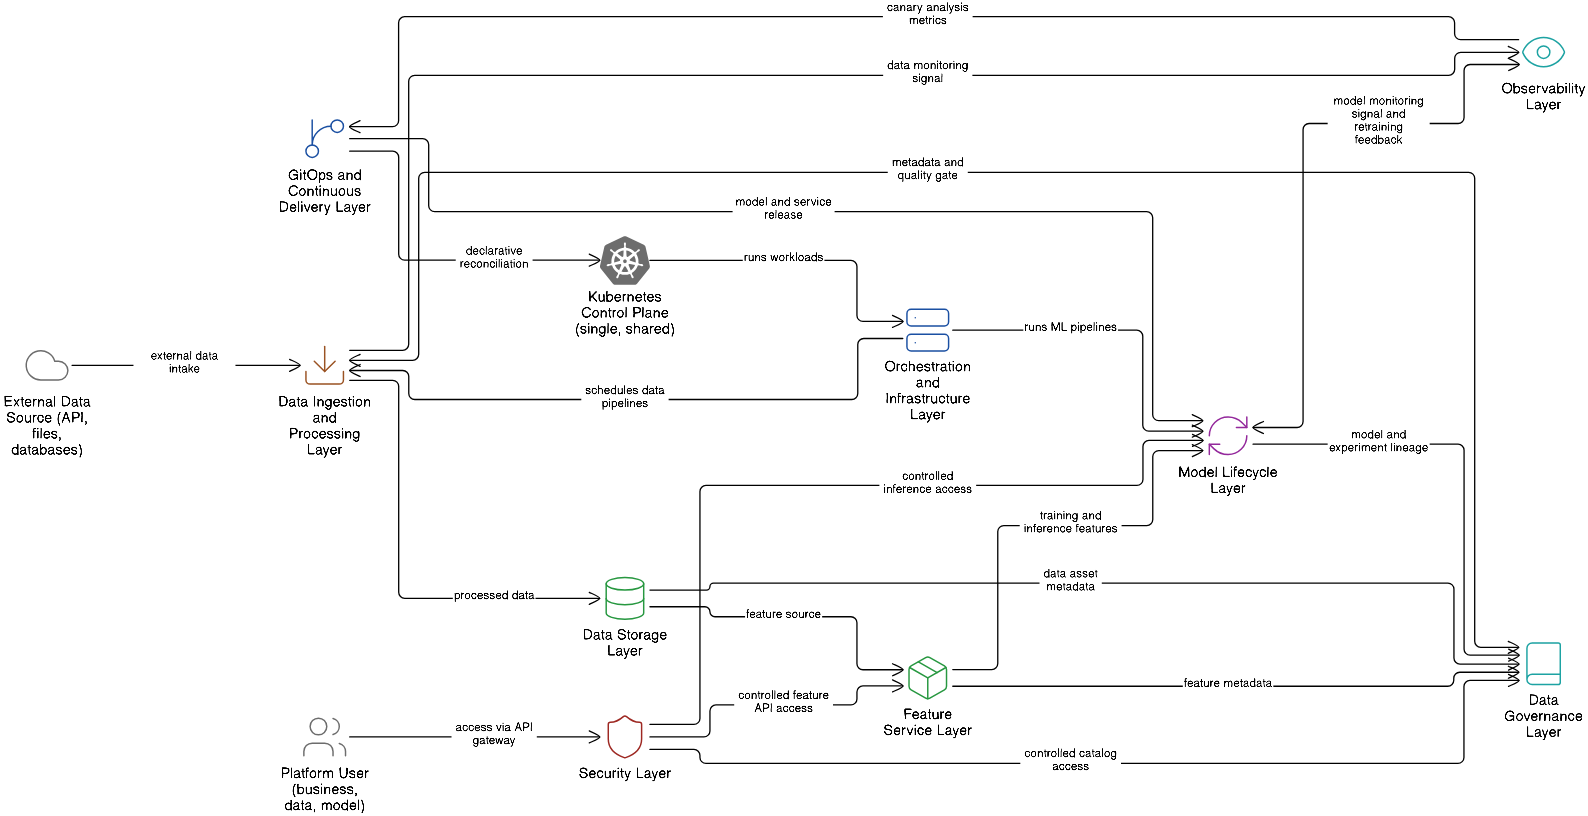
\includegraphics[width=\textwidth]{figures/DataOps_MLOps_Flow.png}
\caption{Integrated service architecture on a shared Kubernetes control plane, drawn without binding to any tool \cite{googlecloud2024mlops}}
\label{fig:architecture}
\end{figure*}

\subsection{Joining the Two Disciplines}
\label{subsec:bridges}

Fig.~\ref{fig:architecture} shows the nine layers as one architecture. DataOps and MLOps meet at three points, and at each one the producing and the consuming side read the same definition rather than two copies of it.

The first is the feature contract. Feast binds the offline store and the online store to one feature definition, so the pipelines that write features and the training and inference code that read them use the same contract.

The second is open lineage. OpenLineage carries transformation events from both the data orchestrator and the training orchestrator, including the SQL transformation steps inside them, into one metadata catalog. The lineage of a training dataset is then traceable from the same graph that holds the ingestion assets.

The third is the declarative control plane. Argo CD reconciles the manifests of both disciplines from one Git repository, so policy and component versions stay consistent across the two. It is also what makes the drift loop of Section~\ref{subsec:drift} declarative.

\subsection{Drift Detection and Retraining}
\label{subsec:drift}

Drift detection sits where the two disciplines meet, because drift is observed on the data layer while its consequence is executed on the model layer. A detector runs as a scheduled job, every 15 minutes for volatile features and hourly for more stable ones. It reads a current window and a reference window from ClickHouse and computes the Population Stability Index with adaptive binning and the Kolmogorov-Smirnov statistic with per-feature thresholds \cite{reis2016kdd}. Scores are written back to an analytics table in ClickHouse for audit, and pushed to Prometheus for alerting.

A scheduled Argo CronWorkflow reads those scores and decides whether to trigger training. Thresholds live in a Git-committed ConfigMap, and each run records a checksum of the configuration version, so a policy change is auditable without inspecting the cluster. When a threshold is crossed, the workflow calls the training pipeline, which assembles its training set through a point-in-time join and logs the run to the model registry as a new version.

Whether that candidate replaces the running model is decided at canary promotion on live serving metrics, not by a separate comparison before deployment. Promotion is configured to halt and roll back when a metric crosses its threshold.

\subsection{Dual-Store Feature Service}
\label{subsec:feature}

The dual-store design is two stores under one contract. ClickHouse holds offline features for training, Valkey serves online lookups at inference, and both derive their schema from the same Feast definition. Vector embeddings are handled separately. Qdrant stands outside Feast as a vector index reached through its native client, because an approximate nearest neighbour load needs memory for the HNSW graph \cite{malkov2020efficient} and behaves differently from a key-value point lookup. Separating them lets each be tuned on its own.

Point-in-time correctness is enforced through the historical feature join, which admits only values whose event timestamp does not exceed each entity row's reference timestamp and still falls inside the feature view's time-to-live. Training therefore sees the values that would have been available at that instant, which is what prevents the optimistic evaluation that leakage produces \cite{kaufman2012leakage}. Batch and stream pipelines write to stores registered on the same feature view, so a consumer does not need to know which pipeline produced a value.
